%-----------------------------------------------------------------------------
%
%               Template for sigplanconf LaTeX Class
%
% Name:         sigplanconf-template.tex
%
% * <soojison96@gmail.com> 2016-05-25T14:17:00.417Z:
%
% ^.
% Purpose:      A template for sigplanconf.cls, which is a LaTeX 2e class
%               file for SIGPLAN conference proceedings.
%
% Guide:        Refer to "Author's Guide to the ACM SIGPLAN Class,"
%               sigplanconf-guide.pdf
%
% Author:       Paul C. Anagnostopoulos
%               Windfall Software
%               978 371-2316
%               paul@windfall.comtian'yan'z
%
% Created:      15 February 2005
%
%-----------------------------------------------------------------------------


\documentclass[numbers]{sigplanconf}

% The following \documentclass options may be useful:

% preprint      Remove this option only once the paper is in final form.
% 10pt          To set in 10-point type instead of 9-point.
% 11pt          To set in 11-point type instead of 9-point.
% numbers       To obtain numeric citation style instead of author/year.

\usepackage{amsmath}
\usepackage{enumerate}
\usepackage{url}
\usepackage{listings}
\usepackage{color}
\usepackage{graphicx}

\definecolor{dkgreen}{rgb}{0,0.6,0}
\definecolor{gray}{rgb}{0.5,0.5,0.5}
\definecolor{mauve}{rgb}{0.58,0,0.82}
\lstset{frame=tb,
  language=Java,
  aboveskip=3mm,
  belowskip=3mm,
  showstringspaces=false,
  columns=flexible,
  basicstyle={\small\ttfamily},
  numbers=none,
  numberstyle=\tiny\color{gray},
  keywordstyle=\color{blue},
  commentstyle=\color{dkgreen},
  stringstyle=\color{mauve},
  breaklines=true,
  breakatwhitespace=true,
  tabsize=2
}

\DeclareGraphicsExtensions{.png,.pdf}
\newcommand{\cL}{{\cal L}}

\begin{document}

\special{papersize=8.5in,11in}
\setlength{\pdfpageheight}{\paperheight}
\setlength{\pdfpagewidth}{\paperwidth}

\conferenceinfo{CONF 'yy}{Month d--d, 20yy, City, ST, Country}
\copyrightyear{2016}
\copyrightdata{978-1-nnnn-nnnn-n/16/05}
\copyrightdoi{nnnnnnn.nnnnnnn}

% Uncomment the publication rights you want to use.
%\publicationrights{transferred}
\publicationrights{licensed}    % this is the default
%\publicationrights{author-pays}

\titlebanner{CSC395 Final Project}        % These are ignored unless
\preprintfooter{Project Proposal}% 'preprint' option specified.

\title{SmartGwent}
\subtitle{}

\authorinfo{Jianting Chen}
           {Grinnell College}
           {chenjian@grinnell.edu}
\authorinfo{Medha Gopalaswamy}
           {Grinnell College}
           {gopalasw@grinnell.edu}
\authorinfo{Eli Most}
           {Grinnell College}
           {mosteli@grinnell.edu}

\maketitle

%\section{Requirements : 3-5 Pages}
%\begin{itemize}
%\item An introduction introducing the problem that the project is trying to solve.
%\item A prior work section describing prior approaches towards solving this problem.
%\item An examples section demonstrating the salient features of your project through examples.  Use pictures and graphs whenever appropriate!
%\item A system section describing the architecture of your system in more detail.  You should give a complete account of your system (e.g., if you built a language, you should describe the full language).  You should also highlight major features of the implementation, e.g., what machine learning algorithms you used (if applicable), as well as libraries that you used.
%\item A reflection section describing the pros and cons of the programming language, tools, and libraries, that you used to build your project.  What aspects of Haskell, Elm, etc. were more productive or more enjoyable to use?  What did you find particularly troublesome or burdensome to do with these languages?
%\end{itemize}


\section{Introduction}
A natural extension of building games for humans to play is to give computers the ability to play these games themselves. The building of a game is a complex issue, including the display of the interface for players, the mechanics of the game, and its content. Humans may build their own strategies for playing this type of game, and often these strategies grow as humans learn from one another. The task of having a computer intelligently play a game, on the other hand, greatly depends on the quality of the game. For some games, such as tic-tac-toe, all possible moves can easily be enumerated, such that one assuredly choose the move most likely to lead to victory. For other games such as Go, this sort of enumeration is impossible, though computers are not necessarily without means to intelligently compete against human opponents. Other games place more emphasis on complexity in strategy and randomness. That is, this strategy may have more to do with having a developed sense of the game, making predictions about what the other player knows and does not know, and intelligently choosing when and where to reveal information. 

Gwent, a small card-based game from The Witcher 3, is just complex enough such that strategy and planning are necessary to competitively play. In Gwent, each player has a deck of cards. The number of cards in each player's deck may vary. Each game consists of up to three rounds. At the start of the first round, each player recieves 10 cards from their deck. In subsequent rounds, the number of cards a player recieves depends on the number of cards the player chose to expend in previous rounds. For example, if a player has a deck of 22 cards, and during the first two rounds of the game this player used 16 cards, then for the third round this player could only have 6 cards. Hence, strategy in Gwent revolves around evaluating opportunity costs. So a strategy may depend on whether the player want to win this round or preserve an advantage for future rounds. Essentially, Gwent rewards players who intelligently cut their losses. To further clarify, a game of Gwent ends when either player has been defeated twice. There is a system of points in Gwent, and if for some round both players end with the same number of points, then there is a draw, which is counted as defeat for both players. There is some additional complexity to Gwent, but the above serves as a general overview.

In this project, we built a simplified version of Gwent with most of the core elements retained. We also attempted to build an AI for the game. 

\section{Prior Work: Artificial Intelligence and Games}
Artificial intelligence algorithms and methods, such as search, pruning, heuristic evaluation functions, and machine learning have been implemented in order to solve many games, including tic-tac-toe, checkers, chess, Reversi, and Go. Some games are completely solved - the computer can enumerate all nodes of the decision tree, and always win, or draw - while others are only partially solved. This could be because the branching factor of the tree is too large, or the information is only partially observable, or there is a probability factor to the game - in any case, while the computer is not guaranteed to win, it has beaten or at least drawn with the human champions of the games in question.

\subsection{Completely Solved Games}
\subsubsection{Tic-Tac-Toe}
Tic-tac-toe is trivially solvable - assuming that both agents play perfectly, the game will always end in a draw. This is one of the simplest applications of artificial intelligence in solving games, and can be achieved with a basic min-max search tree\cite{russell2003artificial}.

\subsubsection{Checkers}
Checkers was solved in 2003, by \textsc{chinook}\cite{schaeffer2007checkers}. However, due to the large search space ($5x10^{20}$), it is only weakly solved, which means that while it can not guarantee a win, it will not lose, and can ensure a draw, at the very least. It is the largest game to be completely solved. \textsc{chinook} uses a database generated with a backward search in combination with tree of current moves, using forward search, an evaluation heuristic, and alpha-beta pruning to determine future moves.

\subsection{Partially Solved Games}
\subsubsection{Chess}
Famous chess computer programs include IBM's \textsc{Deep Mind}, \textsc{Komodo}, and \textsc{Stockfish}. Each program attempts to overcome the large branching factor of chess game trees in a brute force approach, or finding an alternative approach. Past the typical use of traditional methods such as AB-pruning and min-max search, chess computer programs typically include killer heuristics, iterative deepening depth-first search, and others \cite{laramee2000chess}\cite{laramee2000chess2}. 

\subsubsection{Go}
In Go, the 19 by 19 board creates a branching factor far too large for current artificial intelligence techniques to completely solve. While the 5 by 5 board was weakly solved by \textsc{MIGOS} (Mini GO Solver) in 2003\cite{van2003solving}, the full board is yet to be completely solved. \textsc{MIGOS} uses an evaluation function that is a weighted combination of five heuristics, and searches the game tree with an enhanced version of the traditional alpha-beta pruning search, in order to further efficiency of the algorithm. Only recently, in 2016, did a Go program beat a human 9-dan professional on a full board. AlphaGo\cite{silver2016mastering}, is an Go program by Google which, rather in the traditional fashion of using alpha-beta pruning and min-max trees, uses machine learning in the form of deep neural networks, and a Monte Carlo search tree. The use of machine learning and reinforcement learning in the implementation of AlphaGo means that it can learn from previous "experience", whether that be games played against itself, or against human players. This aspect of AlphaGo makes it more generally intelligent, as it has essentially taught itself how to play the game, rather than being hardcoded. Of course our project will not be as advanced, but once we have implemented the basic features of our own SmartGwent, it might be useful to consider implementing a learning aspect to it, especially as card games are very much based on strategy.

\subsection{Card Games}
Many card games involve two aspects that make them harder to solve with traditional artificial intelligence methods, such as AB-pruning and min-max search - imperfect information, and probability. At no point in the game does the computer know where all the cards are, thus making the game a partially observable one, in contrast to the previously mentioned games, which are all fully observable. Therefore, the methods used in attempting to solve card games must take this partially observable environment into consideration. Such methods that can achieve this include Bayesian networks, Monte Carlo search trees, partially observable Markov decision processes, and neural networks\cite{russell2003artificial}.


\subsection{Haskell Binding for Tensorflow}
A popular tool used in the field of machine learning and artificial intelligence is TensorFlow, it features training mathematical models so that it could response in the optimal way. There are some existing Haskell bindings for TensorFlow, such as hTensor and Haskell binding for TensorFlow. However we decided not to move on using TensorFlow, because most of the bindings are still in development and they do not have enough mathematical functions for building appropriate neural nets in SmartGwent.


\section{Examples}

\paragraph{Pipeline}
After drawing their cards,  players play one card per turn unless a Pass is played. Each card has either damage points that will be added to the player's score, or a special ability that affects the board, such as card that draws from the used cards deck. After one player plays Pass, the other player can choose to either keep playing until his or her score exceeds the opponent's, or play a Pass to end the current round.

\begin{figure}
  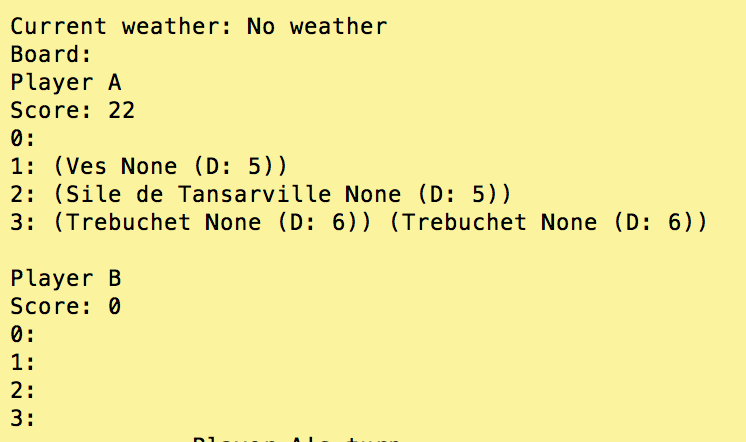
\includegraphics[width=\linewidth]{simpleGameBoard.png}
  \caption{A Simple Board}
  \label{fig:simpleBoard}
\end{figure}

\paragraph{Calculating Scores} 
After each round, SmartGwent will compare the score of each player's cards on the board, and whoever has the higher score wins this round. We use "lives" to tally the number of wins per player, as well as to evaluate the final winner. Each player has two lives in the beginning, and lives are deducted after every loss or draw. Finally, whoever loses all of their lives loses the game. Thus, as a tie leads to a life being deducted, it is possible for both players to lose, e.g. when both players tie twice.

\begin{figure}
  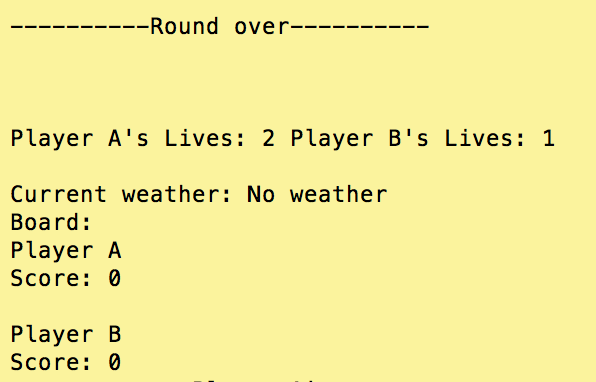
\includegraphics[width=\linewidth]{roundover.png}
  \caption{Round Over, Update Lives}
  \label{fig:roundOver}
\end{figure}

\paragraph{Abilities}
As previously stated, some cards have special abilities that could affect the board or other cards. For example, the Medic ability allows the player to select one card from the used card deck; the Morale ability adds one damage to every other unit in its row; weather abilities reduce the damage of all units in the affected row to one.


\section{System and Architecture}
SmartGwent fully utilizes the modul ability of Haskell and divides the code into different parts. In general, there are two major components to SmartGwent - the game component, that consists of different files that enabled all aforementioned basic game features, and the AI component, where we implemented heuristics and game tree search for the AI player. The code in the former section was organized by the hierarchy of events in the game. From the bottom up, we have turns, and then rounds, which consist of several turns. A game consists of up to three rounds. Static data for the game, such as cards, were organized in a separate section of the project. 
\subsection{Game}
Basic game features are accomplished by functions in the Grammar, Game and Cards folders. Each folder contains Haskell files that 
\paragraph{Grammar} We designed a grammar for SmartGwent in order to make for easier implementation of the game itself. We have two main data structures - Board, and Player. A Board consists of two player, as well as information about the current board, such as the score, the weather (state of the board), the number of rounds left, and the seed used throughout the game to randomize drawing of cards. Each Player contains information specific to that player, such as the cards in their hand, the cards on their side of the board, the cards in their deck, and their used cards, as well as the leader and country of allegiance, and the number of lives they have left. Furthermore, we were able to use Haskell's data types to specify types of Cards (Unit, Weather, Special), to make case analysis on these types of cards easier when implementing evaluate functions.
\subsection{Heuristic and Alpha-Beta Pruning}
The heuristic we implemented was a simpler one, which compares the score of the two players, and attempts to maximize the total score of the AI player. We implemented a variation of min-max search  which kept track of the board state and the value assigned to each possible future board by the heuristic function, and attempted to find the move that best maximized this for the player, and minimized it for the opponent. We found it was difficult to implement a more complex heuristic, especially due to the large branching factor, and the number of different abilities and special cards present. We attempted to counter this by using alpha-beta pruning, but the imperfect information and probabilities continued to prove to be a challenge in implementing a more complex heuristic.

\section{Reflections}
Throughout the implementation, testing and debugging stages, we discovered several advantages and disadvantages of Haskell for developing a game with an AI component. 


\subsection{Algebraic Data Types}
Haskell enabled us to write a convenient grammar for SmartGwent. The structure of the board and the way the game was played was very well suited to representation using Haskell's data types. Record syntax, for example, made handling changes with the state of the game quite convenient, without having to deal with getter and setter boilerplate that might be present in an implementation of Gwent in another language. In addition, when dealing with lists of types, instead of doing many nested if statements, Haskell's pattern matching feature allows us to write elegant code for different cases, making understanding and refactoring our code much easier, especially when adding new features, like different types of Cards. Lastly, by using a typed programming language we found programming SmartGwent to be a smooth process with little time spent debugging, especially during the early stages of development.

\subsection{Hierarchy of Types}
Although Haskell is not a object oriented programming languages, we still found that implementing a hierarchy of cards was easy. Using object oriented terminology, the super class Card has sub classes such as a weather cards (CWeather) and unit cards (CUnit). We are enjoyed the benefits of an object oriented programming languaeg without needing to create a file for every single data type we implemented. Also, we avoided the complicated syntax that most object oriented programming languages have.

\subsection{Dealing with Purity}
Dealing with the IO monad and separating pure code from code wrapped in the IO monad was difficult from a design perspective. At the onset of our project, we failed to recognize and plan ahead for the need for IO. Later on, we realized that at some point we would need to use IO and that some of the core portions of the game relied on having user input. Eventually we were able to overcome this difficulty without too much trouble, partially by storing some IO-related data in the game boards and partially by just getting used to wrapping some aspects of the code in the IO monad. 

\subsection{Testing and Debugging }
Since there is not a well developed IDE for Haskell, we struggled a lot while testing and debugging SmartGwent, especially as the complexity went past simply checking if everything typechecked. Every time we made changes to our code, we would have to run the program again and see if the problem was solved. In addition, because there is no good debugger for Haskell, we often used putStrLn and prettyPrint to debug our program, which isn't the best way to debug, and is potentially dangerous. Still, at some points the type system gave clarity to our coding mistakes, making it easier to refactor and fix bugs.

\subsection{Libraries for Machine Learning}
While we set out to use machine learning, the availability of machine learning resources for Haskell turned out to be scarce. Haskell bindings for TensorFlow were too underdeveloped, with the most relevant neural networks for our project still not implemented. For example, to have an intelligent adversarial agent in Gwent, the agent would have to remember previous cards that were played as part of deciding what to do next. In other words, evaluating the current state of the board would not suffice for thinking intelligently about this game. The types of neural networks which enable this are both not available in the relevant TensorFlow bindings and are too complex to delve into in the context of this course. Other Haskell libraries for different types of machine learning were similarly limited. However, perhaps our goals were too ambitious - using machine learning to build an agent to play a game with incomplete information is still a problem being tackled.

\subsection{Developing a Game in a Functional Language}
Aside from the general conveniences of Haskell, such as algebraic datatypes, there is perhaps little reason to choose Haskell for game development. Games are often quite stateful, which is not so convenient in Haskell. Also, the surrounding resources for using Haskell in games were few. One feature that we planned to implement, a GUI, was sidelined by not having a quick way to use existing libraries to implemement the GUI. For example, in Java we could have used the Swing toolkit to make our GUI quickly. Admittedly, we could have used inline-java to integrate Swing into our game, but we chose to focus on ironing out features of our game and adding the AI.

\subsection{Future Work}
While we made a good deal of progress, there are a number of features that would be enjoyable to add to SmartGwent. First, it would be great to improve the AI so that additional considerations about the different types of cards that can be played are taken into account. Also, it would be good for the AI to be more cognizant of the overall structure of the game in terms of various rounds. In addition, it would be good to have a nice GUI, more options as one starts the game, and the ability to customize one's deck. Playing with another person over the network would also be a great feature to add.

% We recommend abbrvnat bibliography style.
\bibliographystyle{abbrvnat}

% The bibliography should be embedded for final submission.
\bibliography{bibliography}

\end{document}
